\chapter{On Algorithms for Building and Sampling Disordered Crystal States}
\label{ch:iceXI}

% Introduction
	 % Literature Review
% Experiment setup and result
% Future/Ongoing Work (maybe disclude)

\section{States and Properties of Ice}

Ice is cool. 
Ice has many forms, each with unique environments and structures that give rise to similar and unique properties. 

\subsection{Bernal-Fowler Ice Rules}

Bernal-Fowler Ice Rules are the basic rules for how water molecules interact in an ice structure.
DETAILS ON BF PAPER

Basically, water's tetrahedral structure allows for four interactions on each molecule. 
The two protons allow for a hydrogen bond with a lone pair from a neighboring oxygen atom.
Similarly, the oxygen atom's two lone pairs allow for a hydrogen bond with a neighboring proton. 
These rules are fairly rigid in the sense that every water molecule can interact with two oxygen atoms and two protons from four surrounding water molecules.
These are also free-form in the sense that each of the four attached water molecules can occupy one of three rotational microstates, allowing for 81 possible configurations (including rotational duplicates).

\subsection{Forms of Ice}

While ubiquitous in the 'I$_{h}$' form, ice water has many known forms.
As of the writing of this work, there are 17 established forms of ice. 
These forms usually occur in cubic, hexagonal, and orthorhombic crystal structures.
The relationship between external pressure and temperature are the primary defining characteristics of which form will form in a given system. 
Do other characteristics come into play??????? %FIND OUT


\subsection{Ice I$_{h}$}

As the most commonly found form on earth, ice I$_{h}$ is a highly desired form for computational studies involving ice systems. 
%structure
%P/T deets

\subsection{Efforts to Generate Ice I$_{h}$}

Has anyone else published efforts to generate Ice I$_{h}$?
I'm sure someone has.


\subsection{Comparison between Ice XI and Ice I$_{h}$}

While ice I$_{h}$ is known as the most common form of ice found on the planet, it is much more difficult to computationally generate than an ice XI crystal. 
The ease of generation of an ice XI structure stems from the repetition of a unit cell with consistent layering and orientation throughout the crystal lattice. 


With ice I$_{h}$ crystals, the proton-disordered form introduces entropy by way of rotational disorder. 
As the protons and lone pairs are no longer consistently ordered, hydrogen bonds may no longer form properly at all interaction sites. 
The interaction of proton with proton or lone pair with lone pair are not hydrogen bonds and are considered defects in the lattice. 
An ice structure of randomly oriented molecules without consideration of hydrogen bonds will likely produce defects at many interaction sites across the lattice and weaken the integrity of the system, leading to stability problems while running simulations. 
In generating the crystal, the cause of these defects must be considered and countered effectively.

%sub-ish section: necessary attributes to change to convert XI to Ih


\section{Method Design}

% overview
% 0. get pdb ice xi DONE
% 1. read in pdb ice xi
% 2. identify molecules (H2O)
% 3. identify molecule neighbors
% 4. identify corners/edges (in progress)
% 5. for each molecule, identify the tetrahedral spaces
% 6. for each molecule, "randomly" place the two protons
% 7. Check hydrogen bond defect rate
% 8. Fix as necessary (in progress)

\subsection{Overview}

The big idea is to convert an easy-to-make ice XI crystal into an ice Ih crystal.
Because the key difference in structure is the proton-orderedness, it might be possible to rearrange the water molecule orientations in a pseudorandom way to create an ice Ih crystal.
This section walks through the method developed to convert ice XI into ice Ih, the results of initial testing, and imperfections discovered in the design.

\subsection{Selection of Software Tools}

Python was chosen as the language of the tool due to the versatility of the language and the ease of development due to the "pseudocode" written style of the language and the availability of scientific packages including SciPy and NumPy. 
Python version 2.7 was specifically chosen due to familiarity with the language.
Crystal files where defined and saved as Protein Data Bank (.pdb) files as this format allows for defining multiple molecules within a larger structure with a simple X, Y, Z grid position format. 

\subsection{Generation of Source Ice XI}

This is Dr. Fennell's method to create an ice XI pdb file. 
Basically, the ice XI unit cell of eight water molecules is repeated as desired to create a sufficiently large crystal.
The primarily used crystal consists of a 3 x 3 x 6 unit cell repetition totaling 432 water molecules.

\subsection{Source Ingestion}

It is important that the crystal be read and stored in an efficient method to keep relevant information about each molecule easily accessible. 
As the file is read in, each molecule is stored as an entry in a multidimensional array where the first index is the molecule number. 
Further, the second index defines the molecule number where 0 is oxygen and 1 and 2 are the protons. 
The third, fourth, and fifth indices define the X, Y, and Z position coordinates. 

\subsection{Identifying Neighboring Molecules}

Identifying the neighboring molecules proved computationally difficult. 
The most effective method is to find the closest four molecules by computing a distance calculation between every two oxygen atoms.
This ensures every molecule is considered, but also presents significant hurdles.
First, a distance calculation utilizes an extremely computationally-inefficient square root calculation, which can be ignored by instead calculating the squared-distance between molecules and finding the lowest values.

Second, molecules on the walls and edges of the molecule will not have four neighbors in the non-periodic crystal. 
This is accounted for by shifting all six sides to make a pseudo-periodicity for these edge cases. 
Those periodically-neighboring molecules are flagged with a shifting value in the neighboring atom array by specifying a translation in the x, y, or z axis values. 
Unfortunately, the necessary code to implement the periodically-neighboring molecule detections requires a major rewrite of the entire tool and has not yet been implemented.

Once these closest neighboring oxygen atoms have been discovered, the appropriate interacting tetrahedral position is identified by finding the closest of the four tetrahedral positions using the same squared-distance calculation with the four defined tetrahedral positions detailed in the next subsection.

\subsection{Defining Tetrahedral Positions}

An important aspect of pseudorandom selection is the existence of a bank of options. % REWRITE
Using the ingestion portion to calculate and store all tetrahedral possibilities proves useful.
For each water molecule, the first two tetrahedral positions are known by the positions of the two hydrogen atoms. 
The other two positions are found by rotating one hydrogen atom 120$^{\circ}$ twice about the vector from the oxygen atom through the other hydrogen atom and storing the resulting positions as tetrahedral positions three and four. 

This does not produce an exactly correct tetrahedral position of potential hydrogen atoms due to the slight acuteness of the H-O-H bond created by the variance in repulsive forces between the two lone pairs of electrons and two hydrogen atoms. 
% EXACTLY HOW DIFFERENT? 
% WHAT SPECIFIC FORCES?
Fortunately, this difference is sufficiently small for visualization programs like Avogadro to still recognize hydrogen bonds between a rotated hydrogen atom and corresponding neighboring lone pair. 
Currently, the method relies on a very soft annealing process by a simulation package to minimize the effect of this hydrogen bond imperfection. 
% TALKING OUT YOUR ASS. FIND A SOLUTION
Future versions of this method may account for the variations.

\subsection{Pseudorandom Rearrangement of Water Molecules}

Once the tetrahedral positions have been defined, each water molecule is ready to rotate.
What may seem the most crucial step in this methods ends up being the most simple.
As designed, the rotation of water molecules is as simple as using a stepwise iterator to pseudorandomly select two tetrahedral positions for the hydrogen bonds and store the new positions in a new crystal array.
An extremely important note is that this rearrangement does not consider the orientations of neighboring molecules and likely introduces defects of hydrogen - hydrogen and lone pair - lone pair interactions.
The likelihood of a defect-free interaction lattice forming is nearly zero and is assumed to have a great deal of defects within the lattice. 
% PROVE IT?
% SHOW MATH WHY A LOT OF DEFECTS EXIST


\subsection{Detecting Hydrogen Bond Defects}

After all water molecules have been rearranged, defects between incorrectly-interacting hydrogen bonds must be found and corrected.
Discovering the defects relies on the detection of neighboring molecules and the appropriate interacting hydrogen atom or electron lone pair. 
As previously discussed, the initial data ingest records and detects the nearest water molecules and determines the tetrahedral position containing the interacting space, be it electron lone pair or hydrogen atom. 
From that data, the detection of a valid hydrogen bond is as simple as checking both all interacting tetrahedral positions and confirming that they both do not contain or lack a hydrogen atom.
Additionally, each water molecule keeps a count of how many defects are present among the four positions. 
This allows for contextual changes during the correction step.


\subsection{Correcting Hydrogen Bond Defects}

Once the hydrogen bond defects have been discovered and marked, each needs to be corrected.
The most direct approach to this is to sequentially walk through each defect and repeat the pseudorandom rotation until the number of defective regions is zero or a user-specified value.
The current implementation sorts the defect list by the number of defects and attempts to fix the most defective molecules first.
The most defective molecules may include defects impossible to solve by simple rotation, specifically when neighboring molecules have collectively directed three or four hydrogen atoms or electron lone pairs at the target water. 
These can only be solved by adjusting one or more of the neighboring molecules until the number of hydrogen atoms and electron lone pairs have balanced.
Unfortunately, this high-defect problem can quickly escalate if the neighboring molecules contain the same problem of unbalanced hydrogen atoms and electron lone pairs. 
The current solution is to recursively check for and fix these impossible interactions first, but has not yet yielded a defect-free crystal in testing.

The current design of the method allows for the user to specify a threshold of defects as an average per molecule. 
For example, a threshold of 2.5 will allow a maximum of 3 defects on any given molecule and will continue to correct defects until the average number of defects per molecule is equal to or below 2.5.
Because each of these defects will be counted twice, once for each molecule, the total number of defects in a crystal can be determined by multiplying the average defect value by the number of molecules and dividing by two.
As of the current implementation, the method cannot reliably produce a crystal with a threshold below 2 as it will continue to search until the system runs out of available memory and crash without recording any new structure.




\section{Results of Method}

When supplied with an input ice XI crystal, an output structure with rotated water molecule orientations strictly consistent with ice Ih describes a success at the most basic level.
An example before and after of the method is given in figures \ref{fig:iceXI} and \ref{fig:iceIh}.
\begin{figure}
	
	\centering
	
	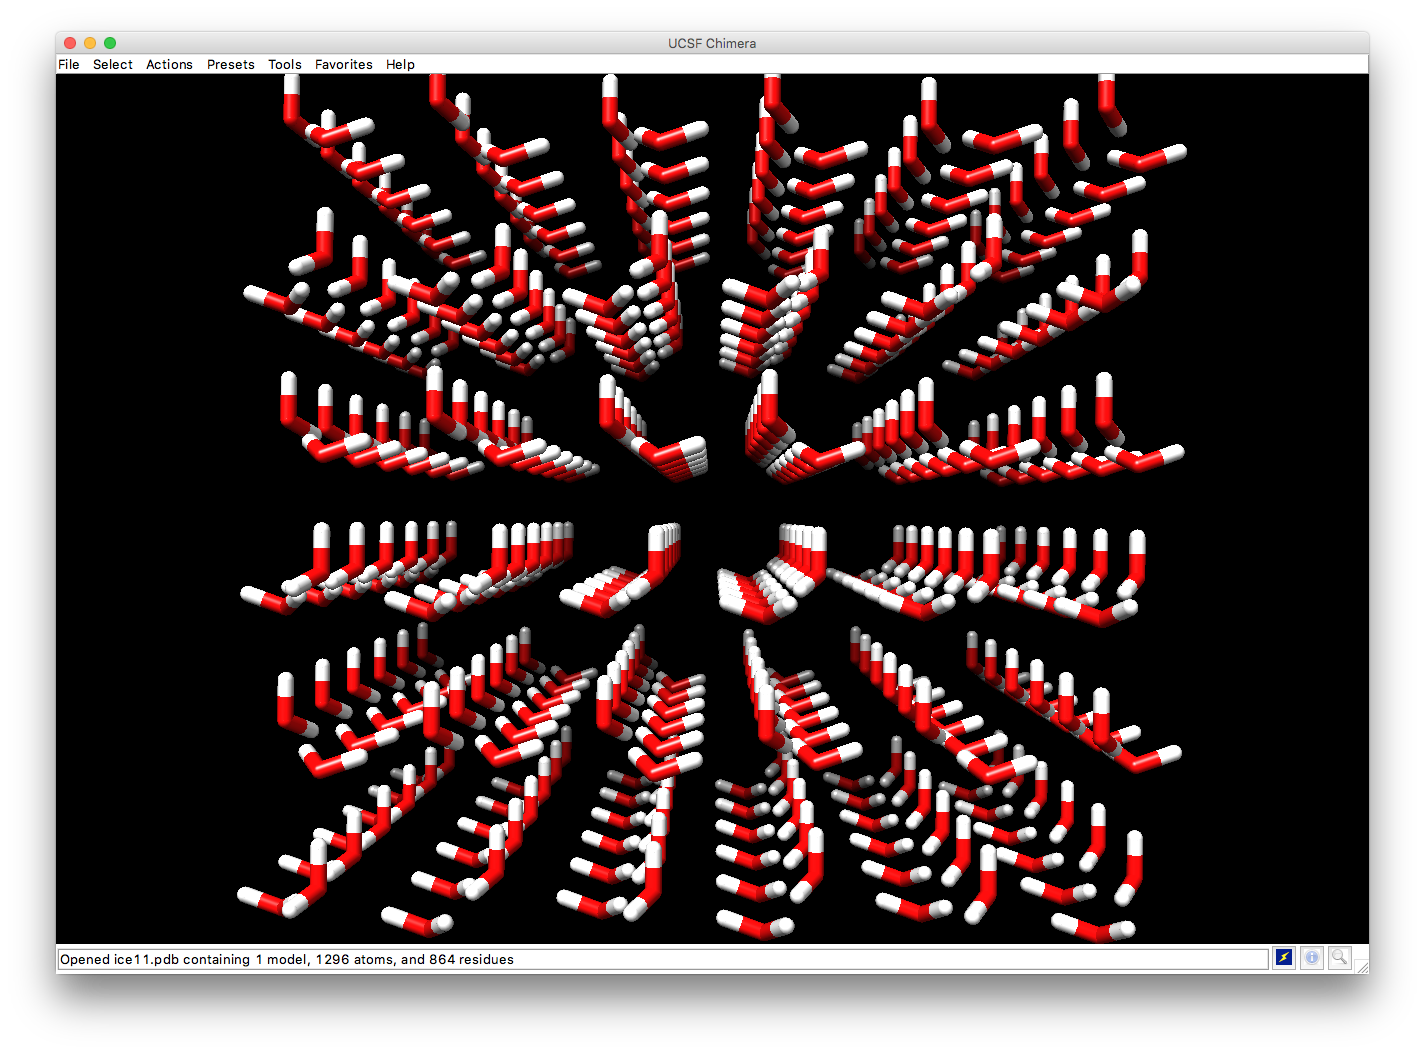
\includegraphics[width=0.75\textwidth]{iceXI.png}
	
	\caption{"Before" image of Ice XI}
	
	\label{fig:iceXI}
	
\end{figure}
\begin{figure}
	
	\centering
	
	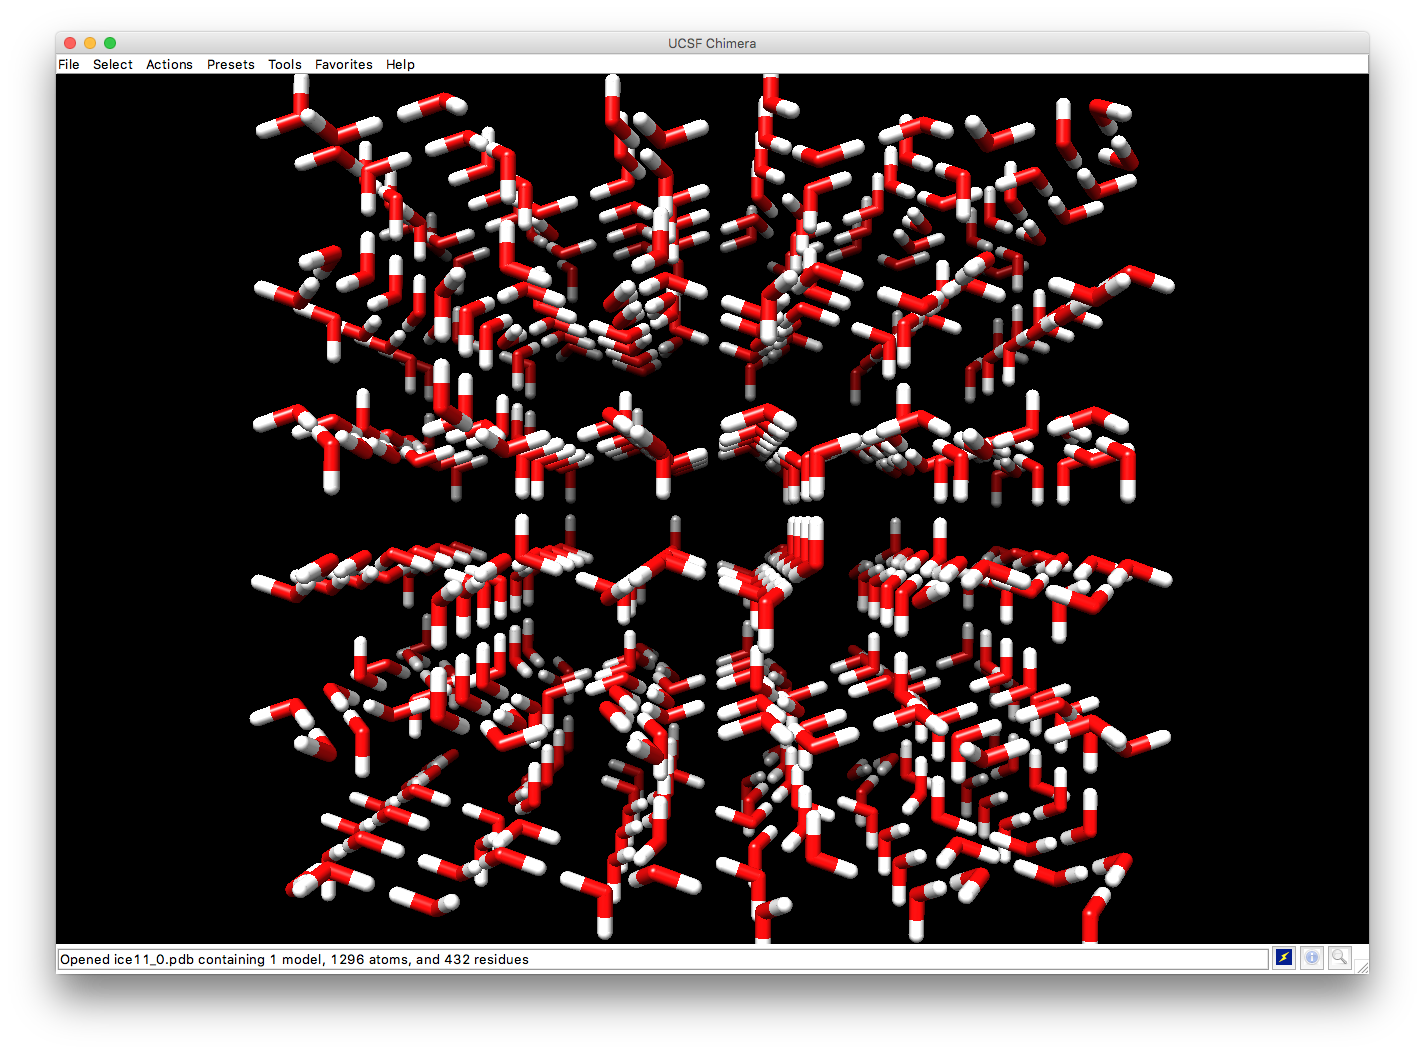
\includegraphics[width=0.75\textwidth]{iceIh.png}
	
	\caption{"After" image of generated ice Ih}
	
	\label{fig:iceIh}
	
\end{figure}
% FIX BELOW
The generated ice Ih has been rotated.
% FIX ABOVE
When following the subsequent layers in the crystal, patterns emerge. 
Inconsistently, some rows of waters remain consistent.
Some of these are a uniform rotation of both hydrogen atoms, while others are just one consistently placed hydrogen atom.
Multiple trials yield internally unique results, yet all contain these strange consistencies.
This may be due to some accidental pattern in the method's implementation.


\section{Comparison with Other Methods}
% USE BUTH PAPER
\subsection{benefits of own method over others}
\subsection{benefits of other methods over this}



\section{Comments on Limitations and Proposed Improvements}

During the hydrogen bond defect correction step, a weakness in the design is that any clustering or regions of high defect density will not be noticed.
This allows the existence of a highly-defective region within the larger structure that could potentially cause problems when the crystal is used in simulations. 
The prevalence and occurrence of these defects have not been studied, but seem a natural inevitability of statistics. 
% SHOW THE STATS
A potential solution with partial development will score regions based on the number of defects as a weighted function expanding out from a central molecule for N connections. 
For example, consider a given molecule defined as level 1. 
The neighboring four molecules are defined as level 2, and continued onward excepting already-defined molecules out to an N$^{th}$ level. 
The number of defects in each level can be counted and averaged.
Then a depressive factor along the lines of $\frac{1}{level}$ can be used to diminish the value of defects further away from the first-level molecule.
This would create a value for each molecule that shows the relative density of defects centered about that specific molecule and could even be plotted as a gradient change within the crystal.
The equation would be something like:
\begin{equation}
Value = \sum_{l=1}^{N_{levels}} \Big[\frac{1}{l} * \frac{1} {N_{molecules}} *\sum_{m=1}^{N_{molecules}}[N_{defects, m}]\Big]
\end{equation}






